\documentclass[10pt]{beamer}

\usetheme[progressbar=frametitle]{metropolis}
\usepackage{appendixnumberbeamer}

\usepackage{booktabs}
\usepackage[scale=2]{ccicons}


\usepackage{pgfplots}
\usepgfplotslibrary{dateplot}

\usepackage{xspace}
\newcommand{\themename}{\textbf{\textsc{metropolis}}\xspace}

\title{Pub Quiz}
\subtitle{Nederlands}
\date{15/07/2019}
\date{}
\author{Slides available at \url{https://sinhp.github.io/blog/}}
\institute{Dizzy}
% \titlegraphic{\hfill\includegraphics[height=1.5cm]{logo.pdf}}
\usepackage{macro}
\usepackage[utf8]{inputenc}
\usepackage[T1]{fontenc}
\usepackage{parskip}
\usepackage{graphicx}
\usepackage{media9}
\usepackage{microtype}

\setbeamertemplate{button}{\tikz
  \node[
  inner xsep=5pt,
  draw=structure!80,
  fill = white, 
  fill=structure!50,
  rounded corners=5pt]  {\color{white}\Large\insertbuttontext};}

\setbeamertemplate{caption}{%
\begin{beamercolorbox}[wd=.3\paperwidth, sep=.5ex]{block body}\color{oranje}{\insertcaption}%
\end{beamercolorbox}%
}

\newcounter{vnum} %% vraag nummer
\newcounter{preframevnum}
\usecounter{vnum}
\newcommand{\vnummer}{\noindent\text{Vraag \arabic{vnum}}\refstepcounter{vnum}}
\setcounter{vnum}{1}

%\pagenumbering{gobble}


\begin{document}

\maketitle

% \begin{frame}{Table of contents}
%   \setbeamertemplate{section in toc}[sections numbered]
%   \tableofcontents[hideallsubsections]
% \end{frame}

\section{Regels}

\begin{frame}[fragile]{Regels}
    \begin{itemize}
        \item Er zijn 14 vragen. Elke vraag heeft een bepaald aantal punten en moet binnen een bepaald maximum tijdslimiet worden beantwoord.
        \item De punten en maximum tijdslimiet van elke vraag worden aangegeven in de rechterbovenhoek. 
        \item Aan het einde tellen we de punten en het team dat meer punten verzamelt wint het spel.
        \item Je kunt geen internet gebruiken.
        \item Je kunt geen encyclopedie gebruiken.
    \end{itemize}
\end{frame}


\section{Vragen: eerste ronde}


\begin{frame}[standout]
 \begin{figure}
     \centering
\includemedia[
        addresource=countdown-short-6.mp3,
        activate=pageopen,
        transparent,
        flashvars={
            source=countdown-short-6.mp3
            &autoPlay=true
            &hideBar=true %enable this to make player invisible
        },
]{
\includegraphics[scale=0.35]{countdown-10.png}}{APlayer.swf}

%https://tex.stackexchange.com/questions/183579/playing-portions-of-mp3-in-pdf?rq=1
% \mediabutton[
%   mediacommand=mysound:play [(10.0)],
%   mediacommand=mysound:pause [(33.0)]
% ]{}

\end{figure}
\end{frame}




\setcounter{preframevnum}{\value{vnum}}
\begin{frame}[fragile]{\vnummer \small  \hfill (\textsc{10 punten}/ \textsc{1 minuut})}
\setcounter{vnum}{\value{preframevnum}}
\pause
\metroset{block=fill}
 \begin{alertblock}{Vraag}
 Noem het nummer en de zanger van het nummer dat het volgende bevat
in de tekst.  \hfill \\
 \pause
 \vspace{10pt}
\texttt{``Want je kunt niets zeker weten en alles gaat voorbij. Maar \ldots''} 
 \end{alertblock}
\pause
\vspace{5pt}
 \begin{exampleblock}{Wenk}
 \vspace{5pt}
 \begin{figure}
     \centering
     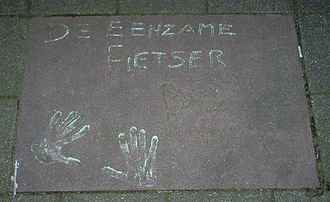
\includegraphics[width=0.4\textwidth, scale=0.6]{WOF_Boudewijn_de_Groot.jpg}
     \caption{\tiny{zijn/haar handafdrukken in de Walk of Fame te Rotterdam}}
     \label{fig:my_label}
 \end{figure}
 \end{exampleblock}
\end{frame}

\setcounter{preframevnum}{\value{vnum}}
\begin{frame}[fragile]{\vnummer \small \hfill (\textsc{10 punten/ 1 minuut})}
\setcounter{vnum}{\value{preframevnum}}
\pause
\metroset{block=fill}
 \begin{alertblock}{Vraag}
   Deze persoon 
   \begin{itemize}
       \item was volgens de Volkskrant Top 200 de invloedrijkste Nederlander van 2007, 2008, en 2009.
       \item is lid van D66.
       \item was eerder rector magnificus van de Erasmus Universiteit. 
       \item is lid van de raad van bestuur van ING.
   \end{itemize}
 \end{alertblock}
\end{frame}


\setcounter{preframevnum}{\value{vnum}}
\begin{frame}[fragile]{\vnummer \small \hfill (\textsc{10 punten/ 1 minuut})}
\setcounter{vnum}{\value{preframevnum}}
\pause
\metroset{block=fill}
 \begin{alertblock}{Vraag}
   Hoe oud is Arjen Lubach?
 \end{alertblock}
\end{frame}


\setcounter{preframevnum}{\value{vnum}}
\begin{frame}[fragile]{\vnummer \small \hfill (\textsc{10 punten/ 1 minuut})}
\setcounter{vnum}{\value{preframevnum}}
\pause
\href{https://embed.vpro.nl/popout/?id=VPWON_1209805&profile=vpro&paused=0&volume=1&muted=0&streaming=0&currenttime=1416}{\beamergotobutton{Finale van WK '74 \scriptsize{\textsc{\color{utrechtBlue}{@vpro.nl}}}}}
\pause
\metroset{block=fill}
 \begin{alertblock}{Vraag}
   welke van deze spelers in de finale van het Wereldkampioenschap voetbal 1974 in West-Duitsland niet tegen Duitsland speelde?  
   \begin{enumerate}
       \item \textsc{Johan Cruijff}
       \item \textsc{Ruud Krol}
       \item \textsc{Piet Schrijvers} 
       \item \textsc{René van de Kerkhof}
       \item \textsc{Arie Haan}
   \end{enumerate}
 \end{alertblock}
%  \begin{figure}[ht!]
%  % using a YouTube video
% \includemedia[
%   width=0.6\linewidth,height=0.3375\linewidth,
%   activate=pageopen,
%   flashvars={
%   modestbranding=1 % no YT logo in control bar
%   &autohide=1 % controlbar autohide
%   &showinfo=0 % no title and other info before start
%   &rel=0 % no related videos after end
% }
% ]{\includegraphics[width=0.6\linewidth]{048}}{https://www.youtube.com/watch?v=slSXVoq75Yg}
% \end{figure}
\end{frame}


\setcounter{preframevnum}{\value{vnum}}
\begin{frame}[fragile]{\vnummer \small \hfill (\textsc{10 punten})}
\setcounter{vnum}{\value{preframevnum}}
\pause
\metroset{block=fill}
 \begin{alertblock}{Vraag}
   Hoe zeg je ``Nederlands'' in het Russich?
 \end{alertblock}
\end{frame}


\setcounter{preframevnum}{\value{vnum}}
\begin{frame}[fragile]{\vnummer \small \hfill (\textsc{10 punten/30 seconden})}
\setcounter{vnum}{\value{preframevnum}}
\pause
\metroset{block=fill}
 \begin{alertblock}{Vraag}
   Hoe zeg je ``Hoe gaat het met jou?'' in het Fries?
 \end{alertblock}
\end{frame}


\setcounter{preframevnum}{\value{vnum}}
\begin{frame}[fragile]{\vnummer \small \hfill (\textsc{10 punten/ 30 seconden})}
\setcounter{vnum}{\value{preframevnum}}
\pause
\metroset{block=fill}
 \begin{alertblock}{Vraag}
   In welke \underline{Grand Prix} van dit jaar eindigde de Nederlandse Formule 1 coureur \underline{Max Verstappen} als eerste na een verschrikkelijke start?
 \end{alertblock}
 \pause
\vspace{10pt}
  \begin{columns}[T,onlytextwidth]
    \column{0.4\textwidth}
    
      \begin{block}{\textsc{A}}
        De Grand Prix Formule 1 van {\color{MyRed3}{Oostenrijk}} 2019
      \end{block}

      \begin{block}{\textsc{C}}
        Grand Prix Formule 1 van {\color{NavyBlue}{Australi\"e}} 2019
      \end{block}
      
    \column{0.4\textwidth}

      \begin{block}{\textsc{B}}
        Grand Prix Formule 1 van {\color{Patina}{Monaco}} 2019
      \end{block}

      \begin{block}{\textsc{D}}
        Grand Prix Formule 1 van {\color{red}{Canada}} 2019
      \end{block}

  \end{columns} 
\end{frame}



\section{Pauze Vraag}

\setcounter{preframevnum}{\value{vnum}}
\begin{frame}[fragile]{\vnummer \small \hfill (\textsc{15 punten/ 1 minuut})}
\setcounter{vnum}{\value{preframevnum}}
\metroset{block=fill}
 \begin{alertblock}{Vraag}
  Hoeveel goals scoorde het Nederlands vrouwenelftal in het WK 2019 in Frankrijk?
 \end{alertblock}
\end{frame}



\setcounter{preframevnum}{\value{vnum}}
\begin{frame}[fragile]{\vnummer \small \hfill (\textsc{10 punten/ 1 minuut})}
\setcounter{vnum}{\value{preframevnum}}
\pause
\metroset{block=fill}
 \begin{alertblock}{Vraag}
   Van welke \texttt{Latijnse naam} was de naam \alert{Utrecht} later afgeleid?
 \end{alertblock}
\end{frame}


\setcounter{preframevnum}{\value{vnum}}
\begin{frame}[fragile]{\vnummer \small \hfill (\textsc{10 punten voor elk/ 1 minuut \& 30 seconden in totaal})}
\setcounter{vnum}{\value{preframevnum}}
\pause
\href{https://scalaleukerleren.nl/taal/educatieve-spelletjes-over-taal/het-spreekwoordenspel/}{\textbf{\texttt{Het Spreekwoorden spel: raad het spreekwoord!}}}\\
\vspace{10pt}
\setcounter{vnum}{\value{preframevnum}}
\texttt{Bijv.}

\begin{columns}[T,onlytextwidth]
    \column{0.5\textwidth}
        \begin{figure}
            \centering
            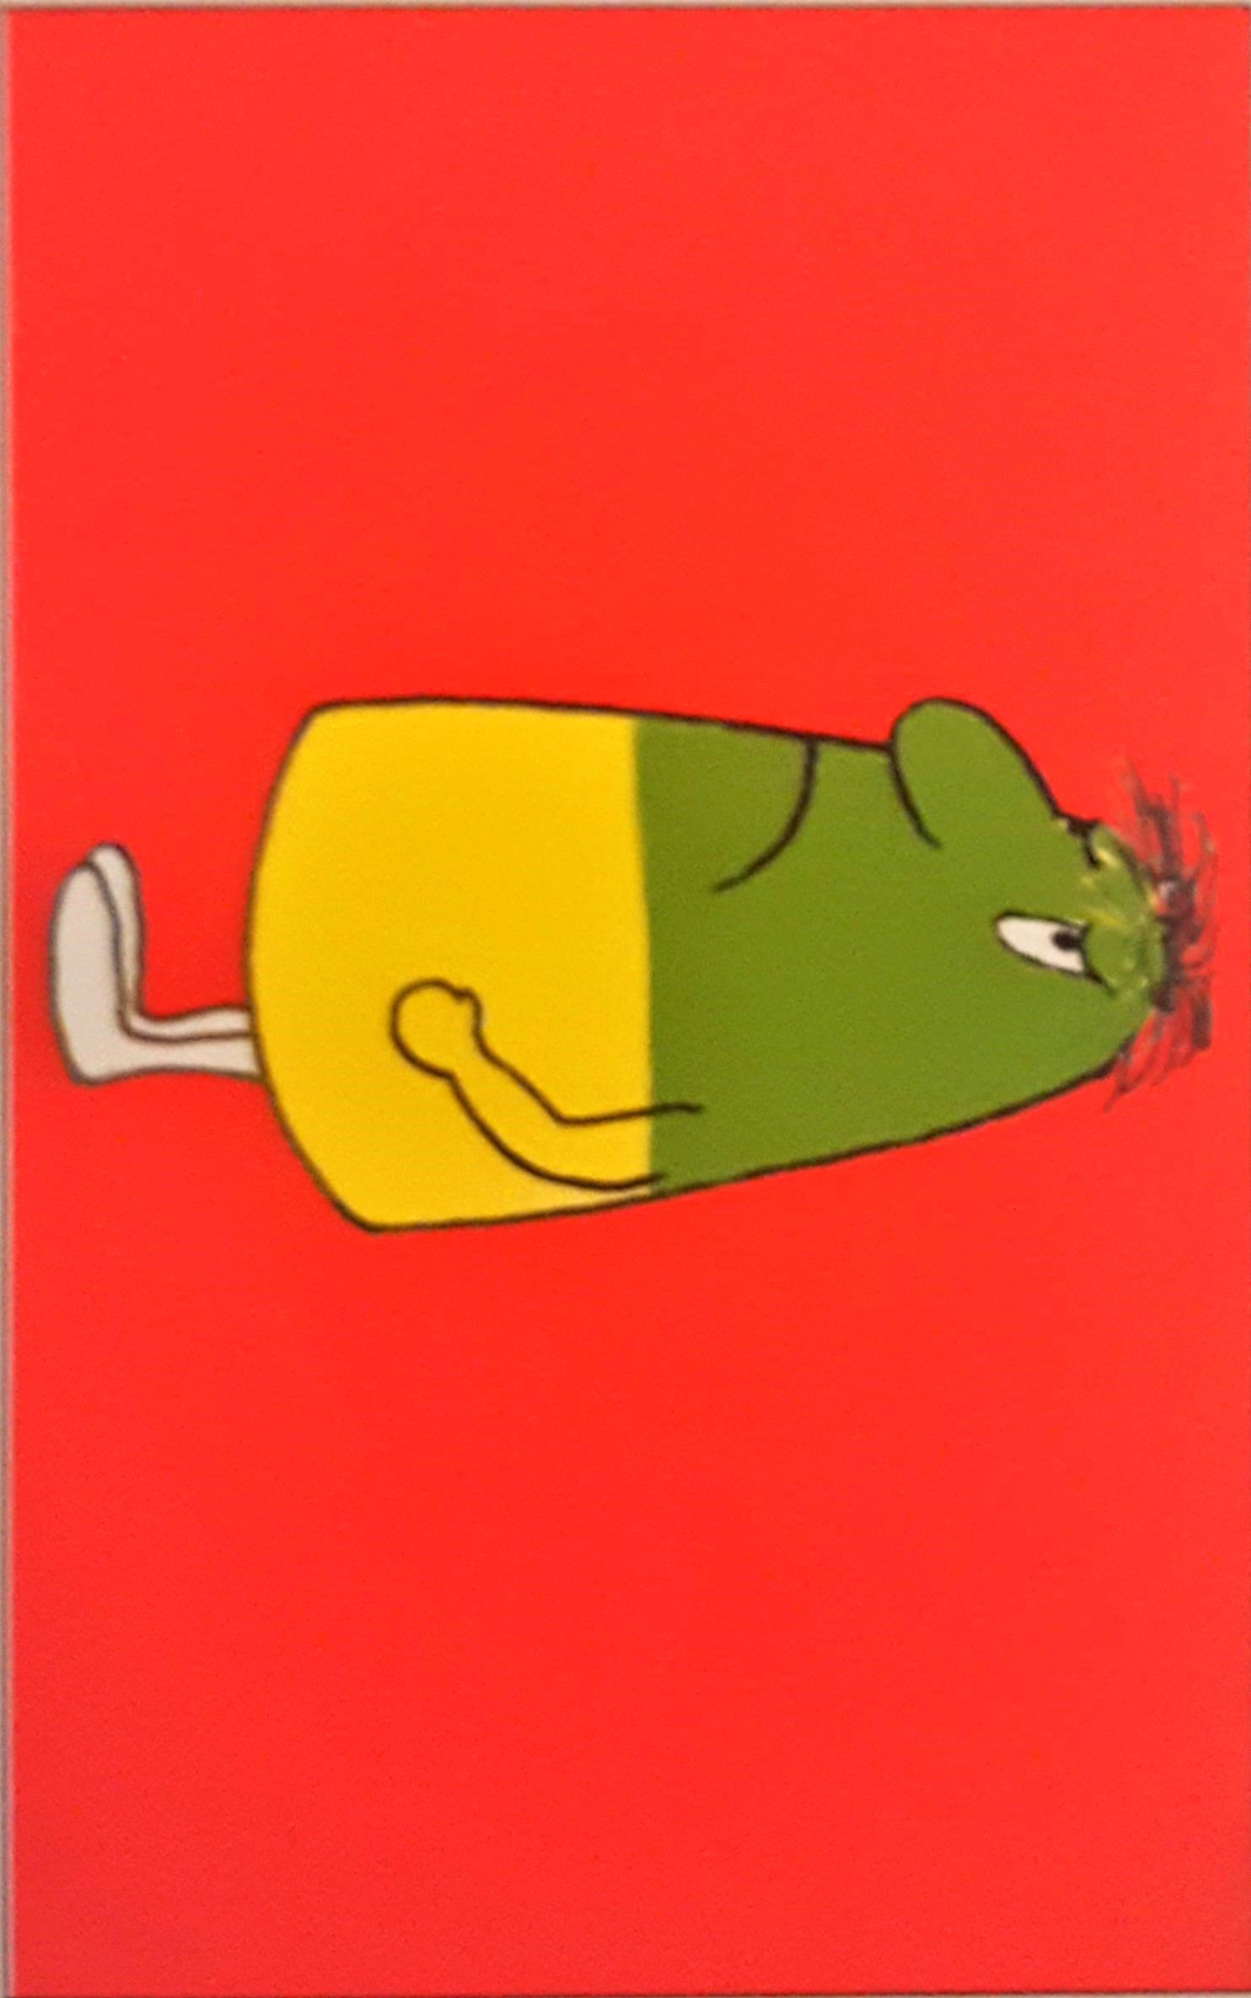
\includegraphics[scale=0.1, angle=90]{groen-en-geel.pdf}
            \caption{Je groen en geel ergeren.}
            \label{}
        \end{figure}
        
    \column{0.5\textwidth}
       \begin{figure}
            \centering
            
\includegraphics[scale=0.1, angle=90]{duim-zuigen.pdf}
            \caption{Iets uit de  duim zuigen.}
            \label{}
        \end{figure}
 \end{columns}
\pause 
\hrule
\hrule
\vspace{10pt}
\begin{columns}[T,onlytextwidth]
    \column{0.5\textwidth}
        \begin{figure}
            \centering
            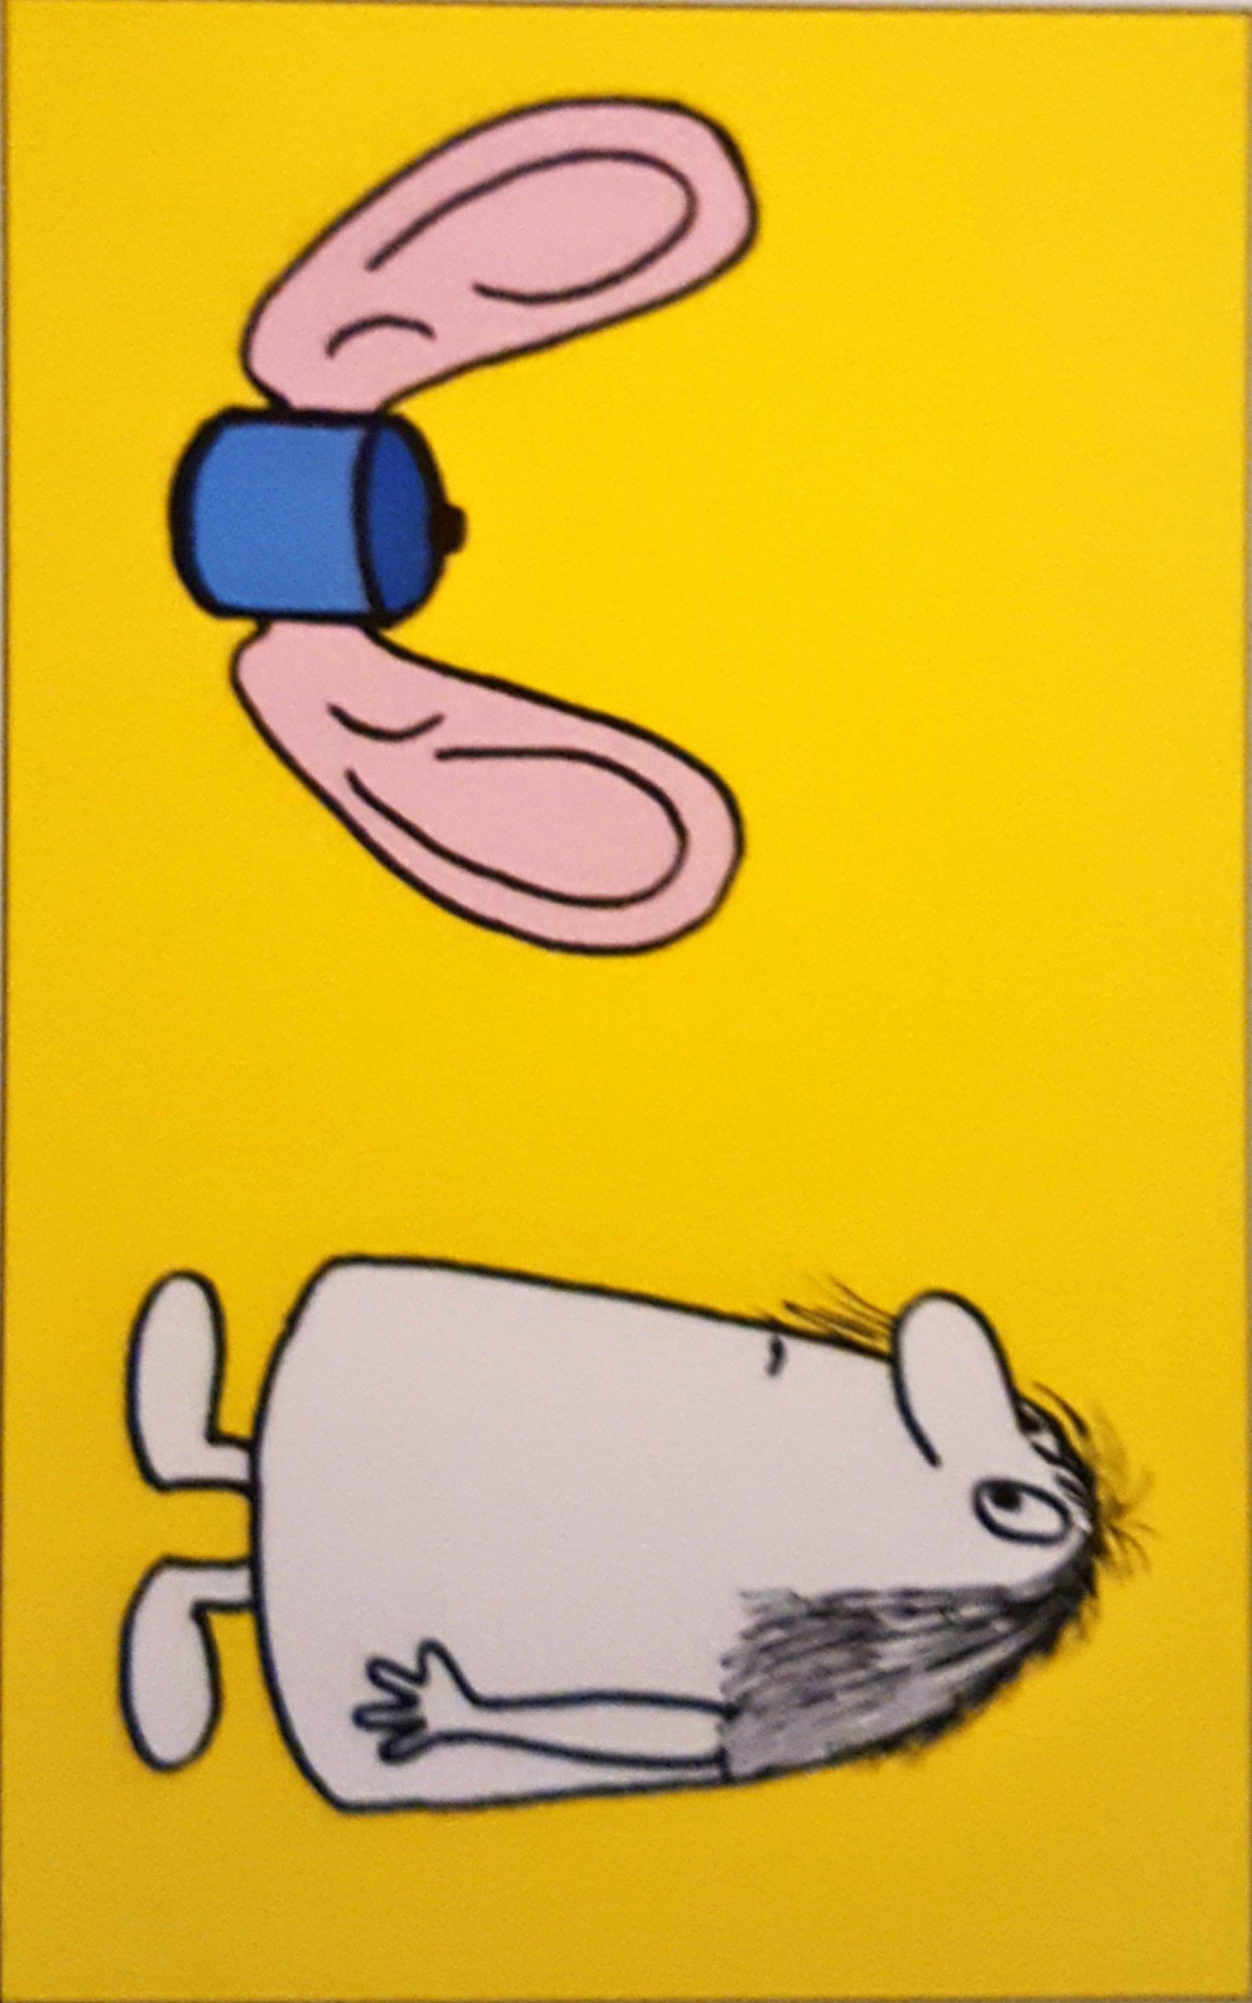
\includegraphics[scale=0.1, angle=90]{kleine-potjes.pdf}
            \caption{\ \ \ \ \ \ \ \ \ \ \ \ ???}
            \label{}
        \end{figure}
        
    \column{0.5\textwidth}
       \begin{figure}
            \centering
            
\includegraphics[scale=0.1, angle=90]{voortouw.pdf}
            \caption{\ \ \ \ \ \ \ \ \ \ \ \ ???}
            \label{}
        \end{figure}
 \end{columns}

\end{frame}



\setcounter{preframevnum}{\value{vnum}}
\begin{frame}[fragile]{\vnummer \small \hfill (\textsc{10 punten voor elk/ 3 minuten in totaal})}
\setcounter{vnum}{\value{preframevnum}}
\pause
\begin{columns}[T,onlytextwidth]
    \column{0.5\textwidth}
        \begin{figure}
            \centering
            
\includegraphics[scale=0.1]{ei-kwijt.jpg}
            \caption{\ \ \ \ \ \ \ \ \ \ \ \ ???}
            \label{}
        \end{figure}
        
    \column{0.5\textwidth}
       \begin{figure}
            \centering
            
\includegraphics[scale=0.096]{lont-ruiken.jpg}
            \caption{\ \ \ \ \ \ \ \ \ \ \ \ ???}
            \label{}
        \end{figure}
 \end{columns}
\pause 
\hrule
\hrule
\vspace{10pt}
\begin{columns}[T,onlytextwidth]
    \column{0.5\textwidth}
        \begin{figure}
            \centering
            
\includegraphics[scale=0.1]{gebakken-lucht.jpg}
            \caption{\ \ \ \ \ \ \ \ \ \ \ \ ???}
            \label{}
        \end{figure}
        
    \column{0.5\textwidth}
       \begin{figure}
            \centering
            
\includegraphics[scale=0.095]{knoop.jpg}
            \caption{\ \ \ \ \ \ \ \ \ \ \ \ ???}
            \label{}
        \end{figure}
 \end{columns}
\end{frame}


\setcounter{preframevnum}{\value{vnum}}
\begin{frame}[fragile]{\vnummer \small \hfill \textsc{(15 punten/ 1 minuut)} }
\setcounter{vnum}{\value{preframevnum}}
\pause
\begin{figure}
    \centering
    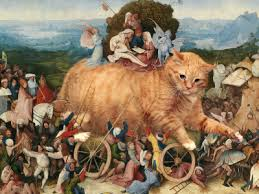
\includegraphics[scale=1.2]{fat-cat-bosch.jpg}
    \caption{\ \ \ \ \ Credit: \href{https://fatcatart.com/2016/03/kitty-fame/?lang=en}{fatcatart}}
    \label{}
\end{figure}
\pause
\metroset{block=fill}
 \begin{alertblock}{Vraag}
   Dit is een licht bewerkt schilderij van Hieronymus Bosch. Wat zit er in plaats van de dikke kat in de originele foto?
 \end{alertblock}
\end{frame}


\setcounter{preframevnum}{\value{vnum}}
\begin{frame}[fragile]{\vnummer \small  \hfill \textsc{(15 punten/ 1 minuut)}}
\setcounter{vnum}{\value{preframevnum}}
\pause
\begin{figure}
    \centering
    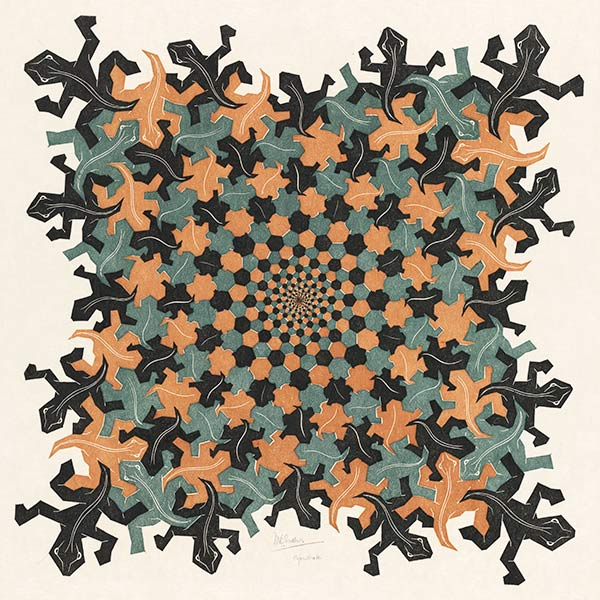
\includegraphics[scale=0.26]{escher-ontwikkeling-ii.jpg}
    \caption{\ \ \ \ \ Credit: \href{https://www.mcescher.nl/galerij/zwitserland-en-belgi/ontwikkeling-iii/}{mcescher.nl}}
    \label{}
\end{figure}
\pause
\metroset{block=fill}
 \begin{alertblock}{Vraag}
   Wat is de naam van dit schilderij van Escher?
 \end{alertblock}
\end{frame}



\setcounter{preframevnum}{\value{vnum}}
\begin{frame}[fragile]{\vnummer \small }
\setcounter{vnum}{\value{preframevnum}}
\pause
\metroset{block=fill}
 \begin{alertblock}{Vraag}
   Wat is het totale aantal punten van de andere team(s) voor deze vraag. Voor elke correcte voorspelling (binnen de marge $\pm 10$) krijgt u 7 extra punten.\\
   \pause
   \vspace{10pt}
   \texttt{bijv. Stel dat er twee teams zijn: team Gandalf en team Saruman. Als team Saruman 60 punten verzamelt voorafgaand aan deze vraag, en team Gandalf schat dat Saruman 50 punten verzamelde voorafgaand aan deze vraag, dan verzamelt Gandalf \underline{extra 10 punten}.} \\
   \vspace{10pt}
   \emph{Vergeet niet dat het maximaal mogelijke aantal punten is \underline{185}.}
 \end{alertblock}
\end{frame}





%%%%%%%%
%%%%%%%%
\section{Einde van vraagen}



%%% -------------
%%% -------------
\section{Antwoorden}
\setcounter{vnum}{1}

\setcounter{preframevnum}{\value{vnum}}
\begin{frame}[fragile]{\vnummer \small \hfill (\textsc{10 punten})}
\setcounter{vnum}{\value{preframevnum}}
\textbf{\texttt{Avond van Boudewijn de Groot}}\\
\vspace{10pt}
\small{\textit{ Nu hoef je nooit je jas meer aan te trekken\\
en te hopen dat je licht het doet.\\
Laat buiten de stormwind nu maar razen in het donker\\
want binnen is het warm en licht en goed.\\
Hand in hand naar buiten kijken waar de regen valt.\\
Ik zie het vuur van hoop en twijfel in je ogen\\
en ik ken je diepste angst.\\
\textbf{\alert{Want je kunt niets zeker weten en alles gaat voorbij.}}\\
Maar ik geloof, ik geloof, ik geloof,\\
ik geloof, ik geloof in jou en mij.\\
En als je 's morgens opstaat ben ik bij je\\
en misschien heb ik al thee gezet.\\
En als de zon schijnt buiten gaan we lopen door de duinen\\
en als het regent gaan we terug in bed.\\
Uren langzaam wakker worden, zwevend door de tijd,\\
ik zie het licht door de gordijnen en ik weet:\\
het verleden geeft geen zekerheid \ldots \\}}
\end{frame}

\setcounter{preframevnum}{\value{vnum}}
\begin{frame}[fragile]{\vnummer \small \hfill (\textsc{10 punten})}
\setcounter{vnum}{\value{preframevnum}}
\textbf{\texttt{Alexander Rinnooy Kan}}\\
\vspace{10pt}
\url{https://www.volkskrant.nl/nieuws-achtergrond/rinnooy-kan-invloedrijkste-nederlander~b61a091d/}
\end{frame}


\setcounter{preframevnum}{\value{vnum}}
\begin{frame}[fragile]{\vnummer \small \hfill (\textsc{10 punten})}
\setcounter{vnum}{\value{preframevnum}}
Arjen Lubach werd geboren op 22 oktober 1979 in Groningen. \\ 
\vspace{10pt}
\begin{center}
  Daarom is hij  \alert{\textbf{\texttt{39 jaar oud}}}.  
\end{center}
\end{frame}

\setcounter{preframevnum}{\value{vnum}}
\begin{frame}[fragile]{\vnummer \small \hfill (\textsc{10 punten})}
\setcounter{vnum}{\value{preframevnum}}
Onder leiding van Rinus Michels werd de finale gehaald, waarin het Nederlandse team van West-Duitsland verloor met 2-1, ondanks een geweldige prestatie.\\
\vspace{5pt}
\pause 
\begin{figure}
\centering
    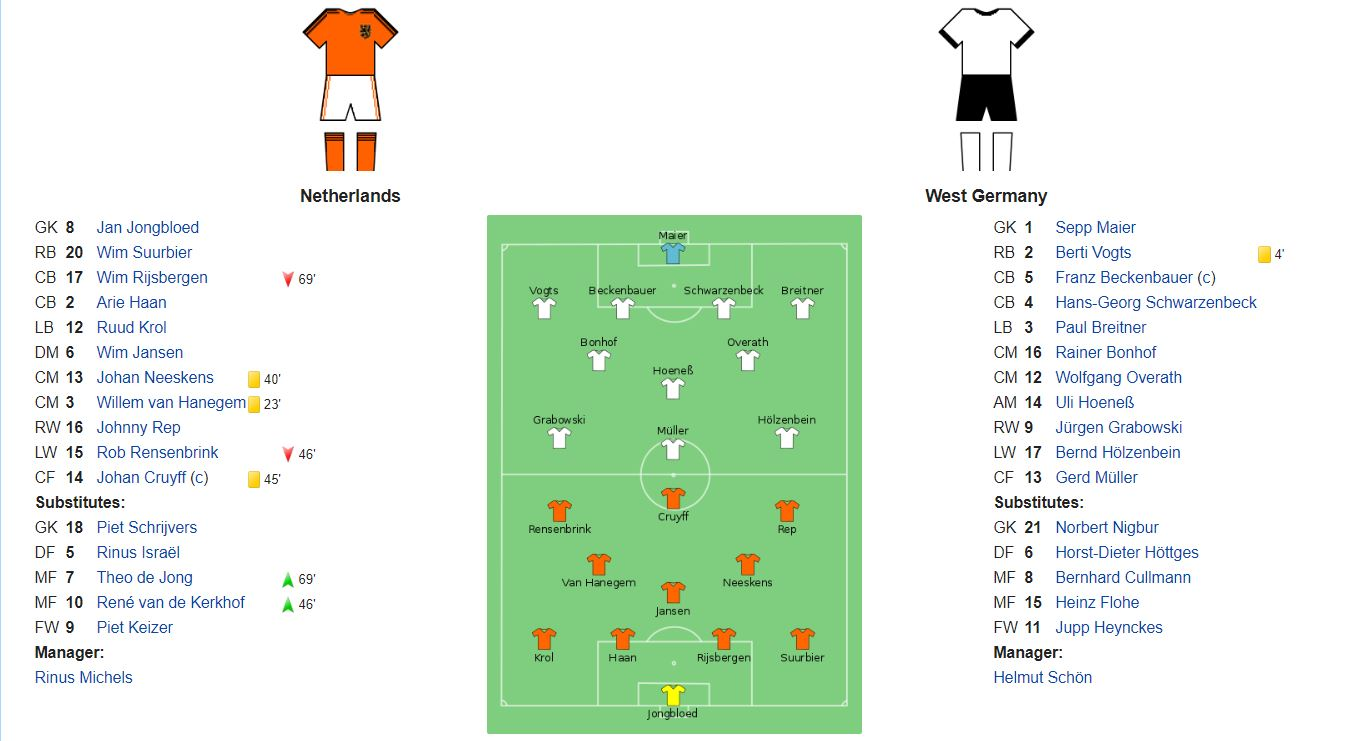
\includegraphics[scale=0.32]{Duitsland-vs-Nederland.JPG}
\end{figure}
\pause
De Aantwoord is \alert{Piet Schrijvers}. Hij was de reserve keeper. \\ 
\end{frame}


\setcounter{preframevnum}{\value{vnum}}
\begin{frame}[fragile]{\vnummer \small \hfill (\textsc{10 punten})}
\setcounter{vnum}{\value{preframevnum}}
\begin{center}
  \alert{\textbf{\texttt{Goll\'andskij}}} 
\end{center}
\end{frame}


\setcounter{preframevnum}{\value{vnum}}
\begin{frame}[fragile]{\vnummer \small \hfill (\textsc{10 punten})}
\setcounter{vnum}{\value{preframevnum}}
\begin{center}
  \alert{\textbf{\texttt{Hoe giet it mei dy?}}}  
\end{center}
\end{frame}


\setcounter{preframevnum}{\value{vnum}}
\begin{frame}[fragile]{\vnummer \small \hfill (\textsc{10 punten})}
\setcounter{vnum}{\value{preframevnum}}
\href{https://www.youtube.com/watch?v=CVuR1UolYJ0&feature=youtu.be&t=55}{De Grand Prix Formule 1 van {\color{MyRed3}{Oostenrijk}} 2019}
\end{frame}


\setcounter{preframevnum}{\value{vnum}}
\begin{frame}[fragile]{\vnummer (Pauze vraag)   \small \hfill (\textsc{10 punten})}
\setcounter{vnum}{\value{preframevnum}}
\begin{center}
  \href{https://www.ekvrouwen.nl/topscorers-wk-voetbal-vrouwen-2019-frankrijk-met-goals-leeuwinnen-nederland/}{\texttt{11 doelpunten}}  
\end{center}

\end{frame}


\setcounter{preframevnum}{\value{vnum}}
\begin{frame}[fragile]{\vnummer \small \hfill (\textsc{10 punten})}
\setcounter{vnum}{\value{preframevnum}}
\alert{\textbf{\texttt{Traiectum}}}
\pause
\vspace{10pt}
\ilum{Onder het huidige Domplein in {\color{utrechtYellow}{Utrecht}} zijn nog resten annwezig van een fort uit de Romeinse tijd. Dat fort, gelegen langs de rivier de Rijn, droeg de Latijnse naam \texttt{Traiectum}, wat `doorwaadbare plaats' (in een rivier) of `overgang' betekent. Van deze naam is later de naam Utrecht afgeleid. \textit{`Utrecht'} is een samenstelling van {\color{utrechtYellow}{\textit{uut}}} (Oudnederlands voor `uit') en {\color{utrechtYellow}{\textit{Trecht}}} (van Traiectum). }
\pause 
\ilum{In 1290, een dichter voegde `uut' toe aan `Trecht'.}
\end{frame}



\setcounter{preframevnum}{\value{vnum}}
\begin{frame}[fragile]{\vnummer \small \hfill (\textsc{elk 10 punten})}
\setcounter{vnum}{\value{preframevnum}}
\vspace{10pt}
\begin{columns}[T,onlytextwidth]
\column{0.45\textwidth}
\ilum{\alert{A: Kleine \underline{potjes} hebben grote \underline{oren}.}\\ 
\vspace{5pt}
{\color{utrechtBlue}{\texttt{DE BETEKENIS:}}} Kinderen  luisteren ook mee, daarom moet je uitkijken met wat je zegt als er kinderen bij zijn.\\
\vspace{5pt}
{\color{utrechtBlue}{\texttt{\scriptsize aanvullende uitleg:}}} \scriptsize{Met kleine potjes zijn hier kinderen bedoeld. Maar echte potjes (bloempotjes) hebben net als kinderen oren. Het woord ``oren'' heeft in dit spreekwoord dus twee betekenissen: gehoororgaan en handvatje.} }
\pause 
\column{0.45\textwidth}
\ilum{\alert{B: Het \underline{voortouw} nemen.}\\ 
\vspace{20pt}
{\color{utrechtBlue}{\texttt{DE BETEKENIS:}}} Het initiatief nemen; ervoor zorgen dat er iets gedaan wordt.\\ 
\vspace{15pt}
{\color{utrechtBlue}{\texttt{\scriptsize aanvullende uitleg:}}} \scriptsize{Een voortouw is enn touw dat aan de voorkant van een schip hangt. Het wordt gebruikt om te schip te verslepen of ann de kade of aan een ander schip vast te leggen. Als je het voortouw neemt, onderneem je dus actie.} }
\end{columns}
\end{frame}

\begin{frame}{Bloempotje}
    \begin{figure}
        \centering
        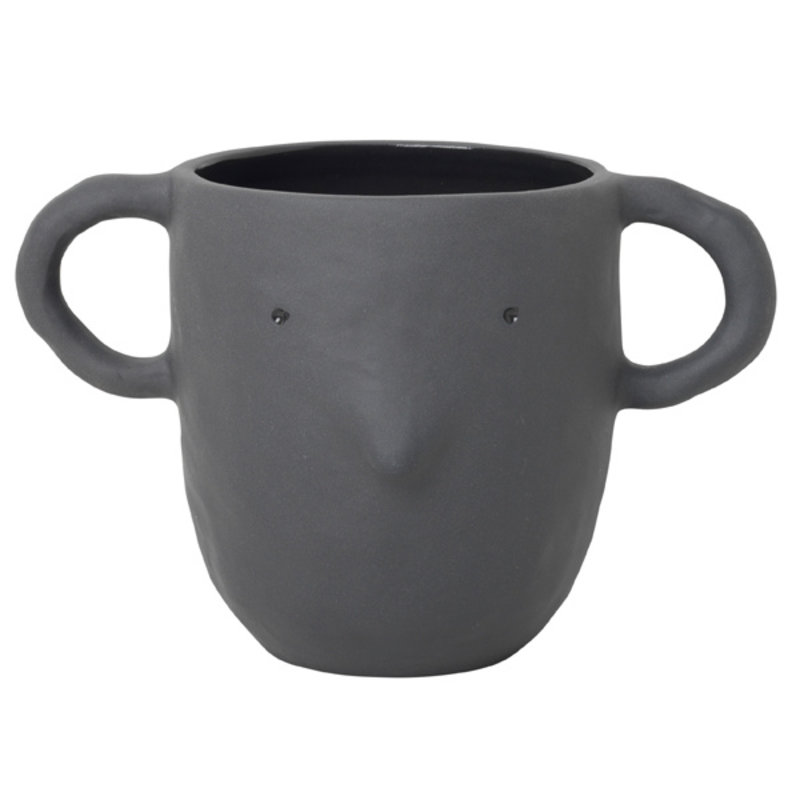
\includegraphics[scale=0.2]{bloempotje.jpg}
        \caption{}
        \label{fig:my_label}
    \end{figure}
\end{frame}


\setcounter{preframevnum}{\value{vnum}}
\begin{frame}[fragile]{\vnummer \small \hfill (\textsc{elk 10 punten})}
\setcounter{vnum}{\value{preframevnum}}
\begin{columns}[T,onlytextwidth]
\column{0.45\textwidth}
\ilum{\alert{A: Je \underline{ei} niet kwijt \underline{kunnen}.}\\ 
\vspace{5pt}
{\color{utrechtBlue}{\texttt{DE BETEKENIS:}}} Niet kunnen doen of zeggen wat je wilt.\\
%\vspace{5pt}
%{\color{utrechtBlue}{\texttt{\scriptsize aanvullende uitleg:}}} \scriptsize{Ei heeft hier de betekenis: iets moet uitgebroed worden. In fit geval gaat het om een idee dat uitgebroed moet worden. Krijg je niet de kans om je idee\"en naar voren te brengen, dan voel je je messtal ongelukkig.} 
}
\vspace{12pt}
\pause
\ilum{\alert{C: \underline{Gebakken} \underline{lucht}.}\\ 
\vspace{5pt}
{\color{utrechtBlue}{\texttt{DE BETEKENIS:}}} Mooie praatjes; zonder betekenis.\\
}
\pause 

\column{0.45\textwidth}
\ilum{\alert{B: \underline{Lont} ruiken.}\\ 
\vspace{10pt}
{\color{utrechtBlue}{\texttt{DE BETEKENIS:}}} Merken dat er iets aan de hand is; merken dat er gevaar is.\\ 
%\vspace{15pt}
%{\color{utrechtBlue}{\texttt{\scriptsize aanvullende uitleg:}}} \scriptsize{Een voortouw is enn touw dat aan de voorkant van een schip hangt. Het wordt gebruikt om te schip te verslepen of ann de kade of aan een ander schip vast te leggen. Als je het voortouw neemt, onderneem je dus actie.} 
}
\pause
\vspace{10pt}
\ilum{\alert{D: In de \underline{knoop} \underline{zitten}.}\\ 
\vspace{5pt}
{\color{utrechtBlue}{\texttt{DE BETEKENIS:}}} In de war zijn; het niet meer weten.\\
}
\end{columns}
\end{frame}


\setcounter{preframevnum}{\value{vnum}}
\begin{frame}[fragile]{\vnummer \small \hfill (\textsc{15 punten})}
\setcounter{vnum}{\value{preframevnum}}
    \begin{center}
        \alert{\texttt{The Haywain Triptych}}
    \end{center}
    \vspace{5pt}
    \begin{figure}
        \centering
        \includegraphics[scale=0.08]{bosch-haywain.jpg}
        \caption{Credit: \href{http://thegolfclub.info/related/haywain-bosch.html}{HAYWAIN BOSCH}}
        \label{}
    \end{figure}
\end{frame}



\setcounter{preframevnum}{\value{vnum}}
\begin{frame}[fragile]{\vnummer \small \hfill (\textsc{15 punten})}
\setcounter{vnum}{\value{preframevnum}}
    \begin{center}
        \alert{\texttt{Ontwikkeling II}},\\
\scriptsize{1939 Houtsnede in bruin, grijs-groen en zwart, gedrukt uit 3 blokken. 455mm x 455mm}
    \end{center}
\end{frame}





%%%------------------------------------------------------------------------------------------------

% \begin{frame}{Tables}
%   \begin{table}
%     \caption{Largest cities in the world (source: Wikipedia)}
%     \begin{tabular}{lr}
%       \toprule
%       City & Population\\
%       \midrule
%       Mexico City & 20,116,842\\
%       Shanghai & 19,210,000\\
%       Peking & 15,796,450\\
%       Istanbul & 14,160,467\\
%       \bottomrule
%     \end{tabular}
%   \end{table}
% \end{frame}



% \begin{frame}{Line plots}
%   \begin{figure}
%     \begin{tikzpicture}
%       \begin{axis}[
%         mlineplot,
%         width=0.9\textwidth,
%         height=6cm,
%       ]

%         \addplot {sin(deg(x))};
%         \addplot+[samples=100] {sin(deg(2*x))};

%       \end{axis}
%     \end{tikzpicture}
%   \end{figure}
% \end{frame}
% \begin{frame}{Bar charts}
%   \begin{figure}
%     \begin{tikzpicture}
%       \begin{axis}[
%         mbarplot,
%         xlabel={Foo},
%         ylabel={Bar},
%         width=0.9\textwidth,
%         height=6cm,
%       ]

%       \addplot plot coordinates {(1, 20) (2, 25) (3, 22.4) (4, 12.4)};
%       \addplot plot coordinates {(1, 18) (2, 24) (3, 23.5) (4, 13.2)};
%       \addplot plot coordinates {(1, 10) (2, 19) (3, 25) (4, 15.2)};

%       \legend{lorem, ipsum, dolor}

%       \end{axis}
%     \end{tikzpicture}
%   \end{figure}
% \end{frame}



% \begin{frame}{Summary}

%   Get the source of this theme and the demo presentation from

%   \begin{center}\url{github.com/matze/mtheme}\end{center}

%   The theme \emph{itself} is licensed under a
%   \href{http://creativecommons.org/licenses/by-sa/4.0/}{Creative Commons
%   Attribution-ShareAlike 4.0 International License}.

%   \begin{center}\ccbysa\end{center}

% \end{frame}

{\setbeamercolor{palette primary}{fg=white, bg=oranje}
\begin{frame}[standout]
  Punten tellen
\end{frame}
}


\end{document}
